\documentclass[11pt]{article}
\usepackage[british]{babel}
\usepackage[T1]{fontenc}
\usepackage[utf8]{inputenc}
\usepackage{amsmath,amssymb,mathpazo}
\renewcommand{\ttdefault}{lmtt}
\usepackage{booktabs}
\usepackage{longtable}
\usepackage{array}
\usepackage{float}
\usepackage[justification=centering]{caption}% for \caption*
\usepackage{graphicx}
\usepackage{xcolor}
\usepackage[a4paper,margin=2.2cm]{geometry}
\usepackage{enumitem}
\usepackage{fancyhdr}
\usepackage{mdframed}
\usepackage{environ}
\usepackage{needspace}
\usepackage{listings}
\usepackage{hyperref}
\hypersetup{colorlinks=true,linkcolor=blue!55!black,linktoc=all,
  pdftitle={Quantitative Research -- Mock Exam 1 -- Solutions},
  pdfauthor={Prof. Dr. Christoph Weisser}}
\sloppy

\definecolor{hsbiblau}{HTML}{3333B2}
\definecolor{hsbiblaudunkel}{HTML}{1C1C6E}
\definecolor{hsbiorange}{HTML}{E69F00}
\definecolor{hsbigrau}{HTML}{9A9A9A}
\definecolor{hsbirot}{HTML}{C0392B}
\definecolor{hsbigruen}{HTML}{2E8B57}

\pagestyle{fancy}
\fancyhf{}
\rhead{\small Quantitative Research}
\lhead{\small Mock Exam 1 -- Solutions and grading key}
\cfoot{\thepage}
\renewcommand{\headrulewidth}{0.4pt}
\setlength{\headheight}{14pt}

\lstdefinestyle{Pystyle}{language=Python, basicstyle=\ttfamily\small,
  keywordstyle=\color{hsbiblau}, commentstyle=\color{hsbigrau!70!black}\itshape,
  stringstyle=\color{teal}, showstringspaces=false, upquote=true,
  columns=fixed, basewidth=0.5em, xleftmargin=1.2em, aboveskip=4pt, belowskip=4pt}
\lstdefinestyle{Pyout}{language={}, basicstyle=\ttfamily\footnotesize,
  keywordstyle={}, commentstyle={}, stringstyle={}, columns=fixed, keepspaces=true,
  basewidth=0.52em, showstringspaces=false, upquote=true, aboveskip=4pt, belowskip=4pt}
\lstset{style=Pystyle}

\newmdenv[linecolor=hsbiblau!70,backgroundcolor=hsbiblau!5,linewidth=0.8pt,
  innertopmargin=6pt,innerbottommargin=8pt,innerleftmargin=9pt,innerrightmargin=9pt,
  skipabove=4pt,skipbelow=8pt]{scenariobox}
\newmdenv[linecolor=hsbirot!70,backgroundcolor=hsbirot!5,linewidth=0.8pt,
  innertopmargin=5pt,innerbottommargin=6pt,innerleftmargin=9pt,innerrightmargin=9pt,
  skipabove=6pt,skipbelow=6pt]{mistakeboxframe}
%% the mistake box is never split: if it does not fit completely on the page,
%% it starts on the next one (no single line / heading at the bottom of a page)
\newsavebox{\mistakeboxmeasure}
\NewEnviron{mistakebox}{\par
  \sbox{\mistakeboxmeasure}{\begin{minipage}{\linewidth}%
    \begin{mistakeboxframe}\BODY\end{mistakeboxframe}\end{minipage}}%
  \Needspace{\dimexpr\ht\mistakeboxmeasure+\dp\mistakeboxmeasure+\baselineskip\relax}%
  \begin{mistakeboxframe}\BODY\end{mistakeboxframe}}
\newmdenv[linecolor=teal!55,backgroundcolor=teal!7,linewidth=0.8pt,
  innertopmargin=5pt,innerbottommargin=7pt,innerleftmargin=9pt,innerrightmargin=9pt,
  skipabove=4pt,skipbelow=8pt]{conceptbox}

%% highlighted final result
\newcommand{\result}[1]{\par\nopagebreak[4]\vspace{2pt}%
  \noindent\fcolorbox{hsbigruen}{hsbigruen!8}{\parbox{0.965\linewidth}{%
  \textbf{Result:}~#1}}\par\nopagebreak[4]\vspace{2pt}}
%% grading rubric of a subtask
\newcommand{\rubric}[1]{\par\nopagebreak[4]\vspace{1pt}%
  \noindent{\footnotesize\textcolor{black!62}{\textbf{Grading (2 P.):} #1}}\par\vspace{2pt}}
%% typical mistake of a subtask (optional)
\newcommand{\mistake}[1]{\par\nopagebreak[4]\noindent{\footnotesize\textcolor{hsbirot!85!black}{\textbf{Typical mistake:} #1}}\par\vspace{4pt}}
\newcommand{\lectureref}[1]{\noindent\textcolor{black!62}{\small$\hookrightarrow$\,\textit{Lecture reference:} #1}\par\vspace{4pt}}

\setlist[enumerate,1]{leftmargin=*}

\title{\vspace{-1.2cm}\textbf{Quantitative Research -- Mock Exam 1}\\[2pt]
\large Solutions, results overview and grading rubric}
\author{Prof.\ Dr.\ Christoph Weisser}
\date{}

\begin{document}
\maketitle
\thispagestyle{fancy}
\vspace{-0.7cm}

\noindent\small\textbf{Structure.} Section~\ref{sec:overview} lists all 30 final results
on one page (quick grading pass). Then, for every subtask, follow the worked solution, the
highlighted final result and a \emph{grading rubric} for the 2 points.\normalsize

\medskip

\vspace{-0.4cm}
\section{Results overview -- all final results at a glance}\label{sec:overview}

\begin{mistakebox}
\small\textbf{Grading note.} Each subtask asks for exactly \emph{one} result: a correct result
with comprehensible working earns 2 points (split for partial answers: see the rubric of the
subtask). A result without working, or correct working with a mere slip (transposed digits,
rounding), counts 1 point. All subtasks are independent -- there are no follow-on errors.
\end{mistakebox}

\begin{footnotesize}
\renewcommand{\arraystretch}{1.0}
\noindent\begin{longtable}{@{}p{0.8cm}>{\raggedright\arraybackslash}p{5.3cm}>{\raggedright\arraybackslash}p{8.4cm}c@{}}
\toprule
\textbf{Part} & \textbf{Asked for} & \textbf{Result} & \textbf{P.}\\
\midrule
\multicolumn{4}{l}{\textbf{Task 1 -- Statistical inference: \texorpdfstring{$z$}{z}-test and confidence interval}\hfill\textnormal{20 points}}\\
\midrule
\textbf{a)} & Hypothesis pair & $H_0\colon \mu = 80$ vs.\ $H_1\colon \mu \neq 80$ & 2\\
\textbf{b)} & Standard error & $\sigma/\sqrt{n} = 12/6 = 2$~EUR & 2\\
\textbf{c)} & Test statistic $Z_n$ & $Z_n = 4.30/2 = 2.15$ & 2\\
\textbf{d)} & Critical value & $z_{1-\alpha/2} = z_{0.975} = 1.96$ & 2\\
\textbf{e)} & Test decision & $|Z_n| = 2.15 > 1.96$ $\Rightarrow$ reject $H_0$ & 2\\
\textbf{f)} & $p$-value & $p = 2\,(1-0.9842) = 0.0316$ & 2\\
\textbf{g)} & $95\,\%$ confidence interval & $84.30 \pm 3.92 = [80.38;\ 88.22]$~EUR & 2\\
\textbf{h)} & Interpretation of the CI & with $95\,\%$ confidence, the mean $\mu$ of \emph{all} orders lies in $[80.38;\ 88.22]$~EUR & 2\\
\textbf{i)} & Type I error in context & rejecting $H_0$ (``mean changed'') although $\mu = 80$~EUR still holds & 2\\
\textbf{j)} & Python command ($t$-test) & \texttt{stats.ttest\_1samp(orders, popmean=80)} & 2\\
\midrule
\multicolumn{4}{l}{\textbf{Task 2 -- Simple and multiple linear regression}\hfill\textnormal{20 points}}\\
\midrule
\textbf{a)} & Slope $\hat\beta_1$ & $\hat\beta_1 = 120/40 = 3$ & 2\\
\textbf{b)} & Intercept $\hat\beta_0$ & $\hat\beta_0 = 60 - 3\cdot 24 = -12$ & 2\\
\textbf{c)} & Interpretation of the slope & $1$\,$^{\circ}$C warmer $\Rightarrow$ on average about $3$ more iced coffees sold & 2\\
\textbf{d)} & Prediction at $x = 25$\,$^{\circ}$C & $\hat y(25) = -12 + 75 = 63$ iced coffees & 2\\
\textbf{e)} & Residual of day 5 & $\hat u_5 = 68 - 72 = -4$ & 2\\
\textbf{f)} & Coefficient of determination $R^2$ & $R^2 = 1 - 40/400 = 0.9$ & 2\\
\textbf{g)} & Correlation coefficient $r_{xy}$ & $r_{xy} = +\sqrt{0.9} = 0.9487$ & 2\\
\textbf{h)} & Python command (OLS) & \texttt{smf.ols("sales \textasciitilde{} temp", data=cafe).fit()} & 2\\
\textbf{i)} & Ceteris-paribus interpretation & holding rain fixed: $+1$\,$^{\circ}$C $\Rightarrow$ on average $3.01$ more iced coffees & 2\\
\textbf{j)} & Significance of \texttt{rain} & $p = 0.253 > 0.05$ $\Rightarrow$ not significant (keep $H_0\colon \beta_2 = 0$) & 2\\
\midrule
\multicolumn{4}{l}{\textbf{Task 3 -- Classification: logistic regression and evaluation}\hfill\textnormal{20 points}}\\
\midrule
\textbf{a)} & Odds of churn & odds $= 0.2/0.8 = 0.25$ & 2\\
\textbf{b)} & Churn probability at $x = 2$ & $\hat\eta = -2$, \ $\hat p = 0.1353/1.1353 = 0.1192$ & 2\\
\textbf{c)} & Interpretation of the odds ratio & each extra call multiplies the \emph{odds} of churn by $1.65$ ($+65\,\%$) & 2\\
\textbf{d)} & Classification at $x = 7$ & $\hat\eta = 0.5 > 0$, $\hat p = 0.6225 > 0.5$ $\Rightarrow$ $\hat y = 1$ (churn) & 2\\
\textbf{e)} & Python command (logit) & \texttt{smf.logit("churn \textasciitilde{} calls", data=df).fit()} & 2\\
\textbf{f)} & Accuracy & $(30 + 140)/200 = 0.85$ & 2\\
\textbf{g)} & Sensitivity & $30/(30 + 10) = 0.75$ & 2\\
\textbf{h)} & Specificity & $140/(140 + 20) = 0.875$ & 2\\
\textbf{i)} & Precision & $30/(30 + 20) = 0.6$ & 2\\
\textbf{j)} & Lower threshold $t = 0.3$ & sensitivity \textbf{increases} (more churners caught) & 2\\
\midrule
\multicolumn{3}{r}{\textbf{Total}} & \textbf{60}\\
\bottomrule
\end{longtable}
\end{footnotesize}

\clearpage

%====================================================================
\section[Task 1 -- Statistical inference: \texorpdfstring{$z$}{z}-test and confidence interval]{Task 1 -- Statistical inference: \texorpdfstring{$z$}{z}-test and confidence interval \hfill\mbox{\normalsize(20 points)}}

\begin{scenariobox}
\textbf{Scenario.} Two-sided $z$-test ($\sigma$ known) of the mean order value of an online shop:
$\mu_0 = 80$~EUR, $\sigma = 12$~EUR, $n = 36$, $\bar x = 84.30$~EUR, $\alpha = 0.05$.
Asked for are the test in its steps, the $p$-value, the $95\,\%$ confidence interval, two
interpretations and the Python command for the $t$-test.
\end{scenariobox}
\lectureref{Part~3, sections \emph{Confidence Intervals} (known variance),
\emph{Hypothesis Tests}, \emph{The $p$-Value} and \emph{Types of Error}; Python: slide
``Hypothesis test with Python -- \texttt{ttest\_1samp}'' and Summary~6.}

\begin{conceptbox}
\textbf{The concepts behind this task}
\begin{itemize}[leftmargin=1.3em,itemsep=1.5pt,topsep=3pt]
\item \textbf{Standard error} ($\sigma$ known): $\mathrm{SE} = \sigma/\sqrt{n}$ -- how strongly $\bar X$ fluctuates around $\mu$.
\item \textbf{Test statistic:} $Z_n = \dfrac{\bar X-\mu_0}{\sigma/\sqrt{n}} \sim N(0,1)$ under $H_0$; two-sided: reject $H_0$ if $|Z_n| > z_{1-\alpha/2}$.
\item \textbf{$p$-value} (two-sided): $p = 2\,\Phi(-|Z_n|)$; reject $H_0$ if $p < \alpha$.
\item \textbf{Confidence interval:} $\text{CI}_{1-\alpha} = \bigl[\bar X \pm z_{1-\alpha/2}\,\sigma/\sqrt{n}\bigr]$; $\mu_0$ outside the CI $\Leftrightarrow$ reject $H_0$ (duality).
\item \textbf{Type~I error:} reject $H_0$ although $H_0$ is true (false alarm); its probability is $\alpha$.
\end{itemize}
\end{conceptbox}

\Needspace{7\baselineskip}
\subsection*{a)\quad Hypothesis pair}
{\interlinepenalty=10000\noindent\textit{The management wants to find out whether the mean order value after the redesign \emph{differs} from the planning figure of $80$~EUR (in either direction). State the hypothesis pair.}\par}\nopagebreak[4]

The statement the management wants to find evidence for -- the mean order value
\emph{differs} from the plan -- goes into $H_1$. Because a deviation in either direction
counts, the test is two-sided:
\[ H_0\colon \mu = 80 \qquad\text{vs.}\qquad H_1\colon \mu \neq 80 . \]
Here $\mu$ is the unknown mean order value of \emph{all} orders after the redesign.
Hypotheses are always statements about the population parameter, never about $\bar x$.
\result{$H_0\colon \mu = 80$ \ vs.\ \ $H_1\colon \mu \neq 80$ \ (two-sided)}
\rubric{1 P. $H_1\colon \mu \neq 80$ (two-sided alternative), 1 P. matching $H_0\colon \mu = 80$.}
\mistake{hypotheses written with $\bar x$ instead of $\mu$, or a one-sided $H_1$ although both directions matter.}

\Needspace{7\baselineskip}
\subsection*{b)\quad Standard error}
{\interlinepenalty=10000\noindent\textit{Compute the standard error $\sigma/\sqrt{n}$ of the sample mean for $\sigma = 12$~EUR and $n = 36$.}\par}\nopagebreak[4]

\[ \mathrm{SE} = \frac{\sigma}{\sqrt{n}} = \frac{12}{\sqrt{36}} = \frac{12}{6} = 2 \text{ EUR}. \]
The mean of $36$ orders fluctuates much less than a single order value: its standard
deviation is only one sixth of $\sigma$.
\result{$\dfrac{\sigma}{\sqrt{n}} = \dfrac{12}{\sqrt{36}} = \dfrac{12}{6} = 2$~EUR}
\rubric{1 P. formula with $\sqrt{36} = 6$, 1 P. result $2$.}
\mistake{dividing by $n$ ($0.33$) or by $\sqrt{n-1}$ instead of $\sqrt{n}$.}

\Needspace{7\baselineskip}
\subsection*{c)\quad Test statistic $Z_n$}
{\interlinepenalty=10000\noindent\textit{Compute the test statistic $Z_n$ for $\bar x = 84.30$~EUR, $\mu_0 = 80$~EUR, $\sigma = 12$~EUR and $n = 36$.}\par}\nopagebreak[4]

\[ Z_n = \frac{\bar x-\mu_0}{\sigma/\sqrt{n}} = \frac{84.30-80}{12/\sqrt{36}}
   = \frac{4.30}{2} = 2.15 . \]
The sample mean lies $2.15$ standard errors \emph{above} the hypothesised value
$\mu_0 = 80$~EUR.
\result{$Z_n = \dfrac{84.30-80}{12/\sqrt{36}} = \dfrac{4.30}{2} = 2.15$}
\rubric{1 P. formula with correct substitution, 1 P. result $2.15$.}

\Needspace{7\baselineskip}
\subsection*{d)\quad Critical value}
{\interlinepenalty=10000\noindent\textit{State the critical value of the two-sided test at the significance level $\alpha = 0.05$ ($\sigma$ known; use Table~1).}\par}\nopagebreak[4]

Two-sided test: $\alpha$ is split into two tails of $\alpha/2 = 0.025$ each, so the
$1-\alpha/2 = 0.975$ quantile is needed. Search $0.9750$ \emph{inside} Table~1: row $1.9$,
column $0.06$, hence
\[ z_{1-\alpha/2} = z_{0.975} = 1.96 . \]
$H_0$ is rejected if $|Z_n| > 1.96$, i.e.\ if $Z_n < -1.96$ or $Z_n > 1.96$.
\result{$z_{1-\alpha/2} = z_{0.975} = 1.96$ \ (reject $H_0$ if $|Z_n| > 1.96$)}
\rubric{1 P. two-sided quantile $z_{1-\alpha/2} = z_{0.975}$ ($\alpha$ split), 1 P. value $1.96$ from the table (also accepted: $\pm 1.96$).}
\mistake{using the one-sided quantile $z_{0.95} = 1.645$.}

\Needspace{7\baselineskip}
\subsection*{e)\quad Test decision}
{\interlinepenalty=10000\noindent\textit{The test statistic is $Z_n = 2.15$ and the critical value is $z_{0.975} = 1.96$. Make the test decision for $H_0\colon \mu = 80$ vs.\ $H_1\colon \mu \neq 80$ at $\alpha = 0.05$.}\par}\nopagebreak[4]

Rejection region of the two-sided test: $|Z_n| > z_{0.975}$. Here
\[ |Z_n| = 2.15 \;>\; 1.96 = z_{0.975} , \]
so the test statistic lies in the rejection region and $H_0\colon \mu = 80$ is rejected at
the $5\,\%$ level. The data provide evidence that the mean order value after the redesign
differs from $80$~EUR -- the sample points to a \emph{higher} value ($\bar x = 84.30$).
\result{Since $|Z_n| = 2.15 > 1.96 = z_{0.975}$, $H_0$ is \textbf{rejected}: the mean order value differs significantly from $80$~EUR.}
\rubric{1 P. comparison $|Z_n| = 2.15 > 1.96$, 1 P. decision ``reject $H_0$''.}

\Needspace{7\baselineskip}
\subsection*{f)\quad $p$-value}
{\interlinepenalty=10000\noindent\textit{Compute the two-sided $p$-value for the test statistic $Z_n = 2.15$ (use Table~1).}\par}\nopagebreak[4]

For $H_1\colon \mu \neq \mu_0$ both tails count:
\[ p = 2\,\Phi(-|Z_n|) = 2\,\bigl(1-\Phi(2.15)\bigr). \]
Table~1, row $2.1$, column $0.05$: $\Phi(2.15) = 0.9842$. Hence
\[ p = 2\,(1-0.9842) = 2\cdot 0.0158 = 0.0316 . \]
Because $p = 0.0316 < 0.05 = \alpha$, the $p$-value leads to the same decision as the
critical value: reject $H_0$. (Python: \texttt{2 * stats.norm.sf(2.15)} gives $0.0316$.)
\result{$p = 2\,\Phi(-|Z_n|) = 2\,\bigl(1-\Phi(2.15)\bigr) = 2\,(1-0.9842) = 0.0316$}
\rubric{1 P. $\Phi(2.15) = 0.9842$ from the table, 1 P. doubling and result $0.0316$.}
\mistake{forgetting the factor $2$ ($0.0158$) or reporting $\Phi(2.15) = 0.9842$ itself.}

\Needspace{7\baselineskip}
\subsection*{g)\quad $95\,\%$ confidence interval}
{\interlinepenalty=10000\noindent\textit{Compute the $95\,\%$ confidence interval for $\mu$ with $\bar x = 84.30$~EUR, $\sigma/\sqrt{n} = 2$~EUR and $z_{0.975} = 1.96$.}\par}\nopagebreak[4]

\[ \text{CI}_{0.95} = \Bigl[\bar x - z_{0.975}\frac{\sigma}{\sqrt n};\ \bar x + z_{0.975}\frac{\sigma}{\sqrt n}\Bigr],
   \qquad e = 1.96\cdot 2 = 3.92 \]
\[ \text{CI}_{0.95} = [84.30-3.92;\ 84.30+3.92] = [80.38;\ 88.22] \text{ EUR}. \]
\emph{Duality:} the planning figure $\mu_0 = 80$ lies \emph{outside} the interval -- this
agrees with the rejection of $H_0\colon \mu = 80$ by the two-sided test at $\alpha = 0.05$.
\result{$84.30 \pm 1.96\cdot 2 = 84.30 \pm 3.92$, \ $\text{CI}_{0.95} = [80.38;\ 88.22]$~EUR}
\rubric{1 P. formula $\bar x \pm z_{0.975}\,\sigma/\sqrt{n}$ (margin of error $3.92$), 1 P. both bounds correct.}

\Needspace{7\baselineskip}
\subsection*{h)\quad Interpretation of the CI}
{\interlinepenalty=10000\noindent\textit{For the mean order value $\mu$, the $95\,\%$ confidence interval $[80.38;\ 88.22]$~EUR was computed. Interpret this interval in one sentence.}\par}\nopagebreak[4]

The lecture gives three correct readings: \emph{coverage} (the procedure yields
intervals that contain the fixed true $\mu$ in $95\,\%$ of all samples), \emph{compatibility}
(the interval holds the values of $\mu$ that are consistent with the data) and
\emph{duality} (it holds exactly the $\mu_0$ a two-sided test at $\alpha = 0.05$ would not reject).

\smallskip
\noindent\emph{Model answer:} ``With $95\,\%$ confidence, the mean order value of all orders
after the redesign lies between $80.38$ and $88.22$~EUR.''

\smallskip
\noindent Not correct: ``$95\,\%$ of the orders lie in the interval'' (the CI is about the
\emph{mean}, not about single orders). Strictly speaking also wrong: ``$\mu$ lies in
\emph{this} interval with probability $95\,\%$'' ($\mu$ is fixed; the bounds are random)
-- 1~P.
\result{With $95\,\%$ confidence, the true mean order value $\mu$ of \emph{all} orders after the redesign lies between $80.38$ and $88.22$~EUR -- intervals constructed in this way contain the true $\mu$ in $95\,\%$ of all samples.}
\rubric{1 P. statement about the true mean $\mu$ of all orders (not about single orders or $\bar x$), 1 P. correct reading of the $95\,\%$ (confidence in the procedure / values compatible with the data).}
\mistake{``$95\,\%$ of all orders have a value between $80.38$ and $88.22$~EUR'' (0 P.).}

\Needspace{7\baselineskip}
\subsection*{i)\quad Type I error in context}
{\interlinepenalty=10000\noindent\textit{Describe in one sentence what a Type~I error would mean in this situation.}\par}\nopagebreak[4]

Type~I error $=$ reject $H_0$ although $H_0$ is true (false alarm):
\[ P(\text{reject } H_0 \mid H_0 \text{ true}) = \alpha = 0.05 . \]
In this situation: the shop concludes that the redesign has changed the mean order value,
although the mean of all orders is in fact still $80$~EUR. Because $H_0$ was rejected here,
a Type~I error is the only error the test can have made. (A Type~II error would be:
keeping $H_0$ although the mean has changed.)
\result{A Type~I error means that the shop concludes that the mean order value has changed (rejects $H_0\colon \mu = 80$) although it is in fact still $80$~EUR -- a false alarm, whose probability is $\alpha = 0.05$.}
\rubric{1 P. ``reject $H_0$ / conclude a change'', 1 P. ``although $H_0$ is true ($\mu = 80$~EUR)'' -- in the context of the order value.}
\mistake{describing the Type~II error (keeping $H_0$ although the mean has changed).}

\Needspace{7\baselineskip}
\subsection*{j)\quad Python command ($t$-test)}
{\interlinepenalty=10000\noindent\textit{In practice $\sigma$ is often unknown. Suppose the 36 order values are stored in a NumPy array \texttt{orders} and $\sigma$ is estimated from the data. Give the \texttt{scipy.stats} command that carries out the two-sided one-sample $t$-test of $H_0\colon \mu = 80$.}\par}\nopagebreak[4]

\begin{lstlisting}
from scipy import stats
res = stats.ttest_1samp(orders, popmean=80)   # two-sided by default
res.statistic, res.df, res.pvalue             # T_n, n - 1 = 35, p-value
\end{lstlisting}
\texttt{ttest\_1samp} estimates $\sigma$ by $s$ and compares $T_n$ with the
$t$-distribution with $n-1 = 35$ degrees of freedom. The default
\texttt{alternative="two-sided"} matches $H_1\colon \mu \neq 80$; one-sided tests would
need \texttt{alternative="less"} or \texttt{"greater"}.
\result{\texttt{stats.ttest\_1samp(orders, popmean=80)}}
\rubric{1 P. function \texttt{stats.ttest\_1samp}, 1 P. arguments \texttt{orders} and \texttt{popmean=80} (also accepted: \texttt{stats.ttest\_1samp(orders, 80)}, the prefix \texttt{scipy.stats.}, with or without \texttt{alternative="two-sided"}).}

\begin{figure}[H]\centering
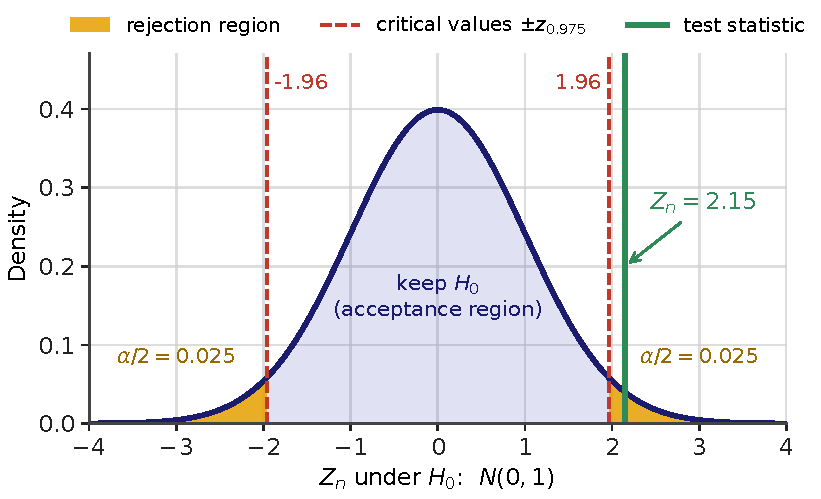
\includegraphics[width=0.62\textwidth]{qrm1_t1_ztest.pdf}
\caption*{\small Standard normal distribution under $H_0$: rejection region $|Z_n| > 1.96$ (orange, $\alpha/2 = 0.025$ per tail) and the observed $Z_n = 2.15$.}
\end{figure}

\begin{figure}[H]\centering
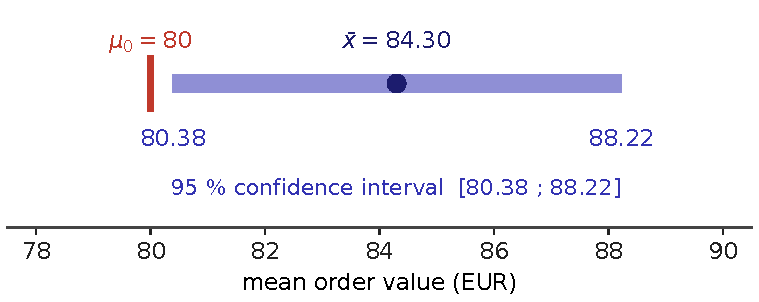
\includegraphics[width=0.70\textwidth]{qrm1_t1_ci.pdf}
\caption*{\small $95\,\%$ confidence interval $[80.38;\ 88.22]$: the planning figure $\mu_0 = 80$ lies outside $\Rightarrow$ reject $H_0$.}
\end{figure}

\begin{mistakebox}
\textbf{Typical mistakes in Task 1}
\begin{itemize}[leftmargin=1.3em,itemsep=1.5pt,topsep=3pt]
\item Using the one-sided quantile $z_{0.95} = 1.645$ for the two-sided test.
\item Forgetting the factor $2$ in the two-sided $p$-value ($0.0158$ instead of $0.0316$).
\item Standard error with $n$ or $n-1$ instead of $\sqrt{n}$.
\item Reading the CI as the range of single order values, or as ``$95\,\%$ probability for \emph{this} interval''.
\item Mixing up the Type~I error (false alarm: reject a true $H_0$) and the Type~II error (miss).
\end{itemize}
\end{mistakebox}
\clearpage

%====================================================================
\section[Task 2 -- Simple and multiple linear regression]{Task 2 -- Simple and multiple linear regression \hfill\mbox{\normalsize(20 points)}}

\begin{scenariobox}
\textbf{Scenario.} Part~A: simple regression of the number of iced coffees sold ($y$) on the daily
maximum temperature ($x$, in $^{\circ}$C), $n = 5$; $\bar x = 24$, $\bar y = 60$,
$S_{xx} = 40$, $S_{xy} = 120$, $S_{yy} = 400$. Part~B: \texttt{statsmodels} output of the
multiple regression \texttt{sales \textasciitilde{} temp + rain} for $n = 60$ days.
\end{scenariobox}
\lectureref{Part~4, sections \emph{Simple Linear Regression} (least squares,
interpretation), \emph{Goodness of Fit: the Coefficient of Determination} and
\emph{Multiple Linear Regression} (ceteris paribus, $t$-test of a coefficient); Python:
Summary~5.}

\begin{conceptbox}
\textbf{The concepts behind this task}
\begin{itemize}[leftmargin=1.3em,itemsep=1.5pt,topsep=3pt]
\item \textbf{OLS estimators:} $\hat\beta_1 = S_{xy}/S_{xx}$, \ $\hat\beta_0 = \bar y - \hat\beta_1\bar x$; \ line $\hat y = \hat\beta_0 + \hat\beta_1 x$.
\item \textbf{Residual:} $\hat u_i = y_i - \hat y_i$ -- positive: point above the line, negative: below.
\item \textbf{Sum-of-squares decomposition:} $\text{TSS} = \text{ESS} + \text{RSS}$, \ $R^2 = \text{ESS}/\text{TSS} = 1 - \text{RSS}/\text{TSS}$.
\item \textbf{Correlation} (simple regression): $R^2 = r_{xy}^2$, so $r_{xy} = \pm\sqrt{R^2}$ with the sign of $\hat\beta_1$.
\item \textbf{Multiple regression:} $\hat\beta_j$ = change of $y$ per unit of $x_j$ \emph{holding the other variables fixed}; $H_0\colon \beta_j = 0$ is rejected if $p < \alpha$.
\end{itemize}
\end{conceptbox}

\Needspace{7\baselineskip}
\subsection*{a)\quad Slope $\hat\beta_1$}
{\interlinepenalty=10000\noindent\textit{Compute the slope $\hat\beta_1$ from $S_{xy} = 120$ and $S_{xx} = 40$.}\par}\nopagebreak[4]

\[ \hat\beta_1 = \frac{S_{xy}}{S_{xx}} = \frac{120}{40} = 3 . \]
The slope has the sign of $S_{xy}$: the cloud of points rises.
\result{$\hat\beta_1 = \dfrac{S_{xy}}{S_{xx}} = \dfrac{120}{40} = 3$ (iced coffees per $^{\circ}$C)}
\rubric{1 P. formula $S_{xy}/S_{xx}$, 1 P. result $3$.}
\mistake{inverted ratio $S_{xx}/S_{xy} = 0.33$.}

\Needspace{7\baselineskip}
\subsection*{b)\quad Intercept $\hat\beta_0$}
{\interlinepenalty=10000\noindent\textit{Compute the intercept $\hat\beta_0$ from $\hat\beta_1 = 3$, $\bar x = 24$ and $\bar y = 60$.}\par}\nopagebreak[4]

\[ \hat\beta_0 = \bar y - \hat\beta_1\,\bar x = 60 - 3\cdot 24 = 60 - 72 = -12 . \]
Estimated line: $\hat y = -12 + 3x$; it passes through the centroid $(\bar x,\bar y) = (24;\ 60)$.
The intercept has no sensible meaning of its own: $x = 0$\,$^{\circ}$C lies far outside the
observed range $20$--$28$\,$^{\circ}$C (extrapolation).
\result{$\hat\beta_0 = \bar y - \hat\beta_1\bar x = 60 - 3\cdot 24 = -12$}
\rubric{1 P. formula $\bar y - \hat\beta_1\bar x$, 1 P. result $-12$ (with sign).}

\Needspace{7\baselineskip}
\subsection*{c)\quad Interpretation of the slope}
{\interlinepenalty=10000\noindent\textit{Interpret the slope $\hat\beta_1 = 3$ in one sentence in the context of the caf\'e.}\par}\nopagebreak[4]

$\hat\beta_1$ is the change of $\hat y$ when $x$ increases by one unit. Here: one degree
Celsius more goes along with, on average, $3$ more iced coffees sold per day. The line
describes an association within the observed range ($20$--$28$\,$^{\circ}$C); it does not
prove a causal effect, and it should not be extended far beyond the data.
\result{On a day that is $1$\,$^{\circ}$C warmer, the caf\'e sells on average about $3$ more iced coffees.}
\rubric{1 P. ``per additional $1$\,$^{\circ}$C'', 1 P. ``on average $3$ more iced coffees''.}
\mistake{no units, or a causal claim (``the heat causes exactly 3 additional sales'').}

\Needspace{7\baselineskip}
\subsection*{d)\quad Prediction at $x = 25$\,$^{\circ}$C}
{\interlinepenalty=10000\noindent\textit{Use the estimated regression line $\hat y = -12 + 3x$ to predict the number of iced coffees sold on a day with a maximum temperature of $x = 25$\,$^{\circ}$C.}\par}\nopagebreak[4]

\[ \hat y(25) = -12 + 3\cdot 25 = -12 + 75 = 63 . \]
$x = 25$ lies within the observed range $[20;\ 28]$, so this is an interpolation -- no
extrapolation problem.
\result{$\hat y(25) = -12 + 3\cdot 25 = 63$ iced coffees}
\rubric{1 P. substitution of $x = 25$, 1 P. result $63$.}

\Needspace{7\baselineskip}
\subsection*{e)\quad Residual of day 5}
{\interlinepenalty=10000\noindent\textit{Compute the residual $\hat u_5$ of day~5 with $(x_5;\ y_5) = (28;\ 68)$, using the estimated regression line $\hat y = -12 + 3x$.}\par}\nopagebreak[4]

\[ \hat y_5 = -12 + 3\cdot 28 = 72, \qquad \hat u_5 = y_5 - \hat y_5 = 68 - 72 = -4 . \]
On day~5 the caf\'e sold $4$ iced coffees fewer than the line predicts; the point lies
\emph{below} the line. (All residuals: $-2,\ 0,\ +2,\ +4,\ -4$; they add up to $0$.)
\result{$\hat y_5 = -12 + 3\cdot 28 = 72$, \ $\hat u_5 = y_5 - \hat y_5 = 68 - 72 = -4$}
\rubric{1 P. fitted value $\hat y_5 = 72$, 1 P. residual $-4$ with the correct sign.}
\mistake{residual with the wrong sign ($\hat y_5 - y_5 = +4$).}

\Needspace{7\baselineskip}
\subsection*{f)\quad Coefficient of determination $R^2$}
{\interlinepenalty=10000\noindent\textit{For the five days, the total sum of squares is $\text{TSS} = 400$ and the residual sum of squares is $\text{RSS} = 40$. Compute the coefficient of determination $R^2$.}\par}\nopagebreak[4]

\[ R^2 = 1 - \frac{\text{RSS}}{\text{TSS}} = 1 - \frac{40}{400} = 0.9
   \qquad\bigl(= \tfrac{\text{ESS}}{\text{TSS}} = \tfrac{360}{400}\ \text{with } \text{ESS} = \text{TSS} - \text{RSS} = 360\bigr). \]
$90\,\%$ of the variation in the daily iced-coffee sales is explained (linearly) by the
temperature; by the rule of thumb of the lecture ($R^2 \ge 0.8$) the fit is good.
Check: $\text{ESS} = \hat\beta_1^2\,S_{xx} = 9\cdot 40 = 360$ \checkmark
\result{$R^2 = 1 - \dfrac{\text{RSS}}{\text{TSS}} = 1 - \dfrac{40}{400} = 0.9$}
\rubric{1 P. formula $1 - \text{RSS}/\text{TSS}$ (or $\text{ESS}/\text{TSS}$ with $\text{ESS} = 360$), 1 P. result $0.9$.}
\mistake{$R^2 = \text{RSS}/\text{TSS} = 0.1$ (share of the \emph{unexplained} variation).}

\Needspace{7\baselineskip}
\subsection*{g)\quad Correlation coefficient $r_{xy}$}
{\interlinepenalty=10000\noindent\textit{Determine the correlation coefficient $r_{xy}$ from $R^2 = 0.9$ and the slope $\hat\beta_1 = 3$.}\par}\nopagebreak[4]

In simple regression $R^2 = r_{xy}^2$, hence
\[ |r_{xy}| = \sqrt{0.9} = 0.9487 , \qquad r_{xy} = +0.9487 \]
-- positive, because the slope $\hat\beta_1 = 3$ is positive. Check with the sums:
$r_{xy} = S_{xy}/\sqrt{S_{xx}S_{yy}} = 120/\sqrt{40\cdot 400} = 120/126.49 = 0.9487$ \checkmark
\result{$r_{xy} = +\sqrt{0.9} = 0.9487$ (positive, because $\hat\beta_1 > 0$)}
\rubric{1 P. $|r_{xy}| = \sqrt{R^2}$, 1 P. value $0.9487$ with positive sign.}
\mistake{$r_{xy} = R^2 = 0.9$, or the sign ignored.}

\Needspace{7\baselineskip}
\subsection*{h)\quad Python command (OLS)}
{\interlinepenalty=10000\noindent\textit{The five days are stored in a pandas DataFrame \texttt{cafe} with the columns \texttt{temp} and \texttt{sales}. Give the \texttt{statsmodels} command that estimates the simple linear regression of \texttt{sales} on \texttt{temp}.}\par}\nopagebreak[4]

\begin{lstlisting}
import statsmodels.formula.api as smf
reg = smf.ols("sales ~ temp", data=cafe).fit()
reg.params             # Intercept -12.0, temp 3.0
\end{lstlisting}
The dependent variable stands to the \emph{left} of \texttt{\textasciitilde}, the explanatory
variable to the right; \texttt{.fit()} carries out the least-squares estimation.
\result{\texttt{smf.ols("sales \textasciitilde{} temp", data=cafe).fit()}}
\rubric{1 P. \texttt{smf.ols(...).fit()}, 1 P. formula \texttt{"sales \textasciitilde{} temp"} (dependent variable on the left) with \texttt{data=cafe} (also accepted: the array form \texttt{sm.OLS(cafe["sales"], sm.add\_constant(cafe["temp"])).fit()}).}
\mistake{formula the wrong way round (\texttt{"temp \textasciitilde{} sales"}) or \texttt{.fit()} forgotten.}

\Needspace{7\baselineskip}
\subsection*{i)\quad Ceteris-paribus interpretation}
{\interlinepenalty=10000\noindent\textit{In the multiple regression of Part~B, the coefficient of \texttt{temp} is $\hat\beta_1 = 3.0055$. Interpret this coefficient in one sentence.}\par}\nopagebreak[4]

In a multiple regression each coefficient is a \emph{partial} effect: it compares
days that differ in temperature but have the \emph{same} rainfall.
\begin{lstlisting}[style=Pyout]
Dep. Variable:                  sales   R-squared:                       0.947
Model:                            OLS   Adj. R-squared:                  0.945
Method:                 Least Squares   F-statistic:                     512.4
                 coef    std err          t      P>|t|      [0.025      0.975]
------------------------------------------------------------------------------
Intercept    -12.2152      3.783     -3.229      0.002     -19.790      -4.641
temp           3.0055      0.131     22.863      0.000       2.742       3.269
rain          -0.4313      0.374     -1.154      0.253      -1.180       0.317
\end{lstlisting}
\emph{Model answer:} ``Holding the rainfall fixed, one degree Celsius more goes along with,
on average, about $3.01$ more iced coffees sold per day.'' The $p$-value $0.000$ shows that
this effect is highly significant.
\result{Holding the rainfall fixed, a $1$\,$^{\circ}$C higher maximum temperature goes along with on average about $3.01$ more iced coffees sold per day.}
\rubric{1 P. ``$+1$\,$^{\circ}$C $\Rightarrow$ on average about $3.01$ (or $3$) more iced coffees'', 1 P. ceteris-paribus clause ``holding the rainfall fixed''.}
\mistake{the clause ``holding rain fixed'' is missing -- then the sentence describes the simple, not the multiple regression.}

\Needspace{7\baselineskip}
\subsection*{j)\quad Significance of \texttt{rain}}
{\interlinepenalty=10000\noindent\textit{In the multiple regression of Part~B, the coefficient of \texttt{rain} is $-0.4313$ with the $p$-value $0.253$ (column \texttt{P>|t|}). Decide at $\alpha = 0.05$ whether rainfall has a significant effect on sales when the temperature is held fixed.}\par}\nopagebreak[4]

$t$-test of a single coefficient: $H_0\colon \beta_2 = 0$ vs.\ $H_1\colon \beta_2 \neq 0$.
Decision rule: reject $H_0$ if $p < \alpha$. Here
\[ p = 0.253 \;>\; 0.05 = \alpha \quad\Rightarrow\quad \text{keep } H_0 . \]
Equivalently, $|t| = 1.154 < t_{0.975;\,57} \approx 2.00$, and the $95\,\%$ CI
$[-1.180;\ 0.317]$ contains $0$. Once the temperature is in the model, the rainfall adds no
significant explanation. This is \emph{confounding}: alone, \texttt{sales \textasciitilde{} rain}
gives a clearly negative slope ($-6.19$), because rainy days are also cooler days.
``Not significant'' does not prove ``no effect'': effects of about $-1$ iced coffee per mm are
still compatible with the data.
\result{$p = 0.253 > 0.05 = \alpha$ $\Rightarrow$ $H_0\colon \beta_2 = 0$ is kept: given the temperature, rainfall has \textbf{no significant} effect on sales.}
\rubric{1 P. comparison $p = 0.253 > 0.05$, 1 P. conclusion ``not significant / keep $H_0$''.}
\mistake{``$p > 0.05$, so rain has no effect at all'' -- not significant only means: no evidence found.}

\begin{figure}[H]\centering
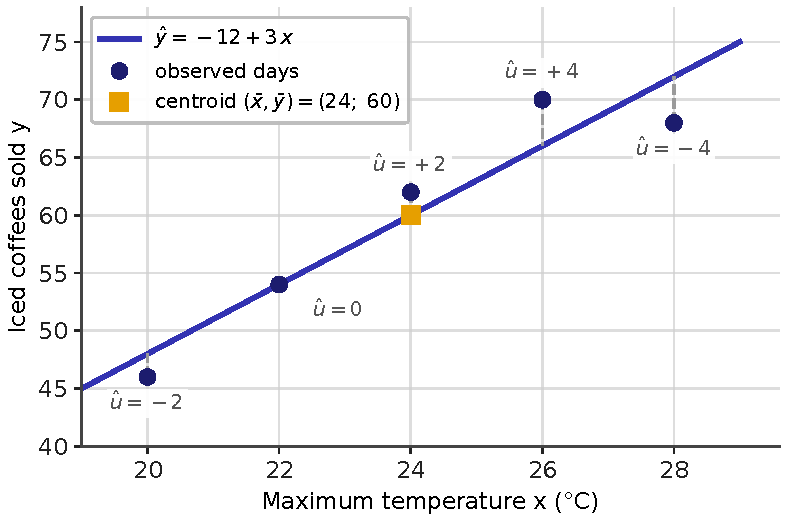
\includegraphics[width=0.62\textwidth]{qrm1_t2_scatter.pdf}
\caption*{\small Scatter plot of the five days with the OLS line $\hat y = -12 + 3x$ and the residuals (dashed); the line passes through $(\bar x,\bar y) = (24;\ 60)$.}
\end{figure}

\begin{mistakebox}
\textbf{Typical mistakes in Task 2}
\begin{itemize}[leftmargin=1.3em,itemsep=1.5pt,topsep=3pt]
\item $\hat\beta_1 = S_{xx}/S_{xy}$ instead of $S_{xy}/S_{xx}$.
\item Residual with the wrong sign ($\hat y_i - y_i$ instead of $y_i - \hat y_i$).
\item $r_{xy} = R^2$, or the sign of $r_{xy}$ ignored.
\item Slope interpreted without units or as a proven causal effect.
\item Multiple regression: the clause ``holding the other variables fixed'' forgotten; ``not significant'' read as ``no effect''.
\end{itemize}
\end{mistakebox}
\clearpage

%====================================================================
\section[Task 3 -- Classification: logistic regression and evaluation]{Task 3 -- Classification: logistic regression and evaluation \hfill\mbox{\normalsize(20 points)}}

\begin{scenariobox}
\textbf{Scenario.} Churn of mobile-phone customers ($Y = 1$) explained by the number $x$ of hotline
calls: $\hat\eta(x) = -3 + 0.5\,x$. Confusion matrix of $n = 200$ test customers at $t = 0.5$:
$\mathrm{TN} = 140$, $\mathrm{FP} = 20$, $\mathrm{FN} = 10$, $\mathrm{TP} = 30$.
\end{scenariobox}
\lectureref{Part~5, sections \emph{Logistic Regression} (odds, log-odds, the model, odds
ratio), \emph{From Probabilities to Decisions} (classification rule) and \emph{Evaluating a
Classifier} (confusion matrix, threshold trade-off); Python: Summary~4.}

\begin{conceptbox}
\textbf{The concepts behind this task}
\begin{itemize}[leftmargin=1.3em,itemsep=1.5pt,topsep=3pt]
\item \textbf{Odds:} $\text{odds} = \dfrac{p}{1-p}$; back: $p = \dfrac{\text{odds}}{1+\text{odds}}$.
\item \textbf{Logistic model:} linear predictor $\eta = \beta_0 + \beta_1 x$ (log-odds), \ $p(x) = \dfrac{e^{\eta}}{1+e^{\eta}}$.
\item \textbf{Odds ratio} $e^{\beta_1}$: factor by which the \emph{odds} change per additional unit of $x$.
\item \textbf{Classification rule:} $\hat y = 1$ if $\hat p(x) > t$; \ $t = 0.5 \Leftrightarrow \hat\eta(x) > 0$.
\item \textbf{Confusion matrix:} accuracy $= (\mathrm{TP}+\mathrm{TN})/n$, sensitivity $= \mathrm{TP}/(\mathrm{TP}+\mathrm{FN})$, specificity $= \mathrm{TN}/(\mathrm{TN}+\mathrm{FP})$, precision $= \mathrm{TP}/(\mathrm{TP}+\mathrm{FP})$.
\end{itemize}
\end{conceptbox}

\Needspace{7\baselineskip}
\subsection*{a)\quad Odds of churn}
{\interlinepenalty=10000\noindent\textit{Last year, $20\,\%$ of all customers churned, i.e.\ $p = 0.2$. Compute the odds of churn.}\par}\nopagebreak[4]

\[ \text{odds} = \frac{p}{1-p} = \frac{0.2}{0.8} = 0.25 . \]
Odds of $0.25$ mean ``$1$ to $4$'': for every customer who churns, four customers stay.
\result{$\text{odds} = \dfrac{p}{1-p} = \dfrac{0.2}{0.8} = 0.25$}
\rubric{1 P. formula $p/(1-p)$, 1 P. result $0.25$.}
\mistake{odds confused with the probability ($0.2$) or computed as $(1-p)/p = 4$.}

\Needspace{7\baselineskip}
\subsection*{b)\quad Churn probability at $x = 2$}
{\interlinepenalty=10000\noindent\textit{Compute the predicted churn probability $\hat p(x)$ of a customer with $x = 2$ hotline calls, using $\hat\eta(x) = -3 + 0.5\,x$ and $e^{-2} = 0.1353$.}\par}\nopagebreak[4]

Pipeline $x \to \hat\eta \to \text{odds} \to \hat p$:
\[ \hat\eta(2) = -3 + 0.5\cdot 2 = -2, \qquad \text{odds} = e^{-2} = 0.1353, \qquad
   \hat p(2) = \frac{0.1353}{1 + 0.1353} = \frac{0.1353}{1.1353} = 0.1192 . \]
A customer with two hotline calls churns with an estimated probability of about $12\,\%$.
\result{$\hat\eta(2) = -3 + 0.5\cdot 2 = -2$, \ $\hat p(2) = \dfrac{e^{-2}}{1+e^{-2}} = \dfrac{0.1353}{1.1353} = 0.1192$}
\rubric{1 P. linear predictor $\hat\eta = -2$, 1 P. probability $0.1192$.}
\mistake{reporting the log-odds $-2$ or the odds $0.1353$ as the probability.}

\Needspace{7\baselineskip}
\subsection*{c)\quad Interpretation of the odds ratio}
{\interlinepenalty=10000\noindent\textit{The odds ratio of the hotline calls is $e^{\hat\beta_1} = e^{0.5} = 1.6487$. Interpret it in one sentence.}\par}\nopagebreak[4]

On the log-odds scale one call more adds $\hat\beta_1 = 0.5$; on the odds scale it
\emph{multiplies} the odds by $e^{0.5} = 1.6487$ -- independent of the starting value of $x$:
\[ \frac{\text{odds}(x+1)}{\text{odds}(x)} = e^{\hat\beta_1} = 1.6487 . \]
\emph{Model answer:} ``Each additional hotline call multiplies the odds of churn by about
$1.65$ (the odds rise by about $65\,\%$).'' The change in the \emph{probability} is not
constant -- it depends on where on the S-curve the customer is.
\result{Each additional hotline call multiplies the \emph{odds} of churn by about $1.65$, i.e.\ the odds of churn rise by about $65\,\%$ per call.}
\rubric{1 P. ``per additional hotline call'', 1 P. ``\emph{odds} multiplied by $1.65$ / $+65\,\%$'' (``probability $+65\,\%$'': 0 P. for this part).}
\mistake{``the probability of churn rises by $65\,\%$'' -- the factor applies to the odds, not to the probability.}

\Needspace{7\baselineskip}
\subsection*{d)\quad Classification at $x = 7$}
{\interlinepenalty=10000\noindent\textit{A customer has $x = 7$ hotline calls. Classify this customer with the threshold $t = 0.5$, using $\hat\eta(x) = -3 + 0.5\,x$ (you may use $e^{0.5} = 1.6487$).}\par}\nopagebreak[4]

\[ \hat\eta(7) = -3 + 0.5\cdot 7 = 0.5, \qquad
   \hat p(7) = \frac{e^{0.5}}{1+e^{0.5}} = \frac{1.6487}{2.6487} = 0.6225 . \]
Since $\hat p(7) = 0.6225 > 0.5 = t$, the customer is classified as \textbf{churner}
($\hat y = 1$). Shortcut: $t = 0.5$ corresponds to $\hat\eta > 0$, and $\hat\eta(7) = 0.5 > 0$.
The decision boundary lies at $\hat\eta = 0 \Leftrightarrow x = 6$: customers with at least
$7$ calls are flagged.
\result{$\hat\eta(7) = 0.5 > 0$, \ $\hat p(7) = \dfrac{1.6487}{2.6487} = 0.6225 > 0.5$ \ $\Rightarrow$ \ $\hat y = 1$: predicted to \textbf{churn}}
\rubric{1 P. $\hat\eta = 0.5$ or $\hat p = 0.6225$, 1 P. classification $\hat y = 1$ (churn).}

\Needspace{7\baselineskip}
\subsection*{e)\quad Python command (logit)}
{\interlinepenalty=10000\noindent\textit{The customer data are stored in a pandas DataFrame \texttt{df} with the columns \texttt{churn} (coded $0/1$) and \texttt{calls}. Give the \texttt{statsmodels} command that estimates the logistic regression of \texttt{churn} on \texttt{calls}.}\par}\nopagebreak[4]

\begin{lstlisting}
import numpy as np
import statsmodels.formula.api as smf
g = smf.logit("churn ~ calls", data=df).fit()
print(g.summary())     # z-tests of the coefficients
np.exp(g.params)       # odds ratios
\end{lstlisting}
\texttt{smf.logit} estimates the coefficients by maximum likelihood; the response must be
coded $0/1$.
\result{\texttt{smf.logit("churn \textasciitilde{} calls", data=df).fit()}}
\rubric{1 P. \texttt{smf.logit(...).fit()} (not \texttt{smf.ols}), 1 P. formula \texttt{"churn \textasciitilde{} calls"} with \texttt{data=df} (also accepted: the array form \texttt{sm.Logit(df["churn"], sm.add\_constant(df["calls"])).fit()}).}
\mistake{\texttt{smf.ols} instead of \texttt{smf.logit} (a linear probability model).}

\Needspace{7\baselineskip}
\subsection*{f)\quad Accuracy}
{\interlinepenalty=10000\noindent\textit{Compute the accuracy of the classifier from the confusion matrix with $\mathrm{TN} = 140$, $\mathrm{FP} = 20$, $\mathrm{FN} = 10$ and $\mathrm{TP} = 30$.}\par}\nopagebreak[4]

\[ \text{accuracy} = \frac{\mathrm{TP}+\mathrm{TN}}{n} = \frac{30 + 140}{200} = \frac{170}{200} = 0.85 . \]
$85\,\%$ of all test customers are classified correctly (error rate $0.15$). Note: the trivial
rule ``nobody churns'' would already reach $160/200 = 0.80$ -- accuracy alone is not enough.
\result{$\text{accuracy} = \dfrac{\mathrm{TP}+\mathrm{TN}}{n} = \dfrac{30 + 140}{200} = 0.85$}
\rubric{1 P. formula $(\mathrm{TP}+\mathrm{TN})/n$, 1 P. result $0.85$.}

\Needspace{7\baselineskip}
\subsection*{g)\quad Sensitivity}
{\interlinepenalty=10000\noindent\textit{Compute the sensitivity of the classifier from the confusion matrix with $\mathrm{TN} = 140$, $\mathrm{FP} = 20$, $\mathrm{FN} = 10$ and $\mathrm{TP} = 30$.}\par}\nopagebreak[4]

Condition on the row ``Actual Yes'' ($40$ actual churners):
\[ \text{sensitivity} = P(\hat y = 1 \mid y = 1) = \frac{\mathrm{TP}}{\mathrm{TP}+\mathrm{FN}} = \frac{30}{30+10} = 0.75 . \]
The rule catches $75\,\%$ of the customers who actually churn.
\result{$\text{sensitivity} = \dfrac{\mathrm{TP}}{\mathrm{TP}+\mathrm{FN}} = \dfrac{30}{40} = 0.75$}
\rubric{1 P. formula $\mathrm{TP}/(\mathrm{TP}+\mathrm{FN})$ (row ``Actual Yes''), 1 P. result $0.75$.}
\mistake{dividing by the column total ``Pred.\ Yes'' ($30/50$ is the precision).}

\Needspace{7\baselineskip}
\subsection*{h)\quad Specificity}
{\interlinepenalty=10000\noindent\textit{Compute the specificity of the classifier from the confusion matrix with $\mathrm{TN} = 140$, $\mathrm{FP} = 20$, $\mathrm{FN} = 10$ and $\mathrm{TP} = 30$.}\par}\nopagebreak[4]

Condition on the row ``Actual No'' ($160$ customers who stay):
\[ \text{specificity} = P(\hat y = 0 \mid y = 0) = \frac{\mathrm{TN}}{\mathrm{TN}+\mathrm{FP}} = \frac{140}{140+20} = 0.875 . \]
$87.5\,\%$ of the loyal customers are correctly left alone.
\result{$\text{specificity} = \dfrac{\mathrm{TN}}{\mathrm{TN}+\mathrm{FP}} = \dfrac{140}{160} = 0.875$}
\rubric{1 P. formula $\mathrm{TN}/(\mathrm{TN}+\mathrm{FP})$ (row ``Actual No''), 1 P. result $0.875$.}
\mistake{$\mathrm{TN}/(\mathrm{TN}+\mathrm{FN}) = 140/150$ (column instead of row).}

\Needspace{7\baselineskip}
\subsection*{i)\quad Precision}
{\interlinepenalty=10000\noindent\textit{Compute the precision of the classifier from the confusion matrix with $\mathrm{TN} = 140$, $\mathrm{FP} = 20$, $\mathrm{FN} = 10$ and $\mathrm{TP} = 30$.}\par}\nopagebreak[4]

Condition on the column ``Pred.\ Yes'' ($50$ flagged customers):
\[ \text{precision} = P(y = 1 \mid \hat y = 1) = \frac{\mathrm{TP}}{\mathrm{TP}+\mathrm{FP}} = \frac{30}{30+20} = 0.6 . \]
$60\,\%$ of the customers flagged as churners really churn -- $4$ of $10$ alarms are false
alarms. Sensitivity and precision both have TP on top but divide by different totals.
\result{$\text{precision} = \dfrac{\mathrm{TP}}{\mathrm{TP}+\mathrm{FP}} = \dfrac{30}{50} = 0.6$}
\rubric{1 P. formula $\mathrm{TP}/(\mathrm{TP}+\mathrm{FP})$ (column ``Pred.\ Yes''), 1 P. result $0.6$.}
\mistake{confusing precision with sensitivity ($30/40$).}

\Needspace{7\baselineskip}
\subsection*{j)\quad Lower threshold $t = 0.3$}
{\interlinepenalty=10000\noindent\textit{To catch more churners, the provider lowers the threshold from $t = 0.5$ to $t = 0.3$. Does the sensitivity increase or decrease?}\par}\nopagebreak[4]

Lowering $t$ flags every customer with $\hat p(x) > 0.3$ instead of $\hat p(x) > 0.5$:
on the log-odds scale $\hat\eta(x) > \log(0.3/0.7) = -0.847$, i.e.\ $x \ge 5$ calls instead of
$x \ge 7$. Every customer flagged before is still flagged, plus some more. Hence
$\mathrm{TP}$ can only rise and $\mathrm{FN}$ only fall:
\[ \text{sensitivity} = \frac{\mathrm{TP}}{\mathrm{TP}+\mathrm{FN}} \ \uparrow \quad(\text{denominator fixed at } 40). \]
The price: more false alarms ($\mathrm{FP}\uparrow$), so the specificity falls. Which threshold
is best is a business decision (cost of a lost customer vs.\ cost of a retention offer).
\result{The sensitivity \textbf{increases} (it cannot decrease): with $t = 0.3$ more customers are classified as churners, so more of the actual churners are caught ($\mathrm{TP}\uparrow$, $\mathrm{FN}\downarrow$).}
\rubric{1 P. ``increases'', 1 P. reason: more customers predicted as churners $\Rightarrow$ more actual churners caught.}
\mistake{``decreases'' -- confusing sensitivity with specificity, which falls when the threshold is lowered.}

\begin{figure}[H]\centering
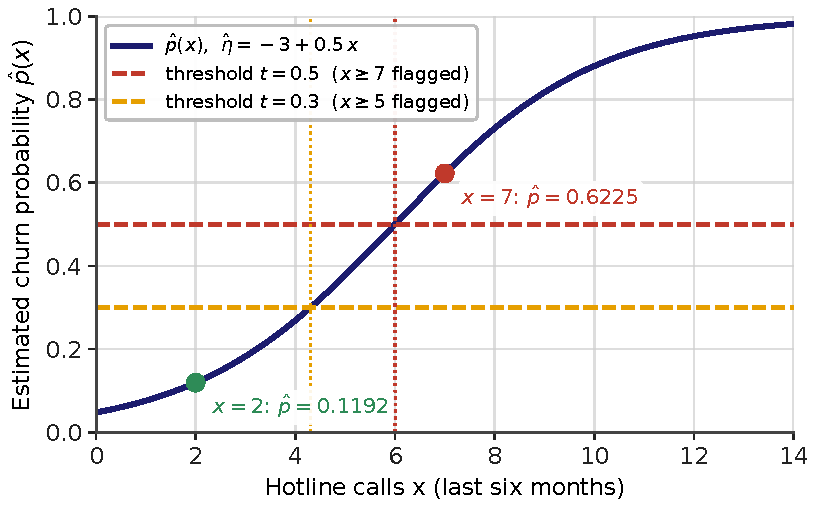
\includegraphics[width=0.62\textwidth]{qrm1_t3_logistic.pdf}
\caption*{\small Estimated churn probability $\hat p(x)$ with $\hat\eta(x) = -3 + 0.5\,x$: customers with $x = 2$ ($\hat p = 0.1192$) and $x = 7$ ($\hat p = 0.6225$); thresholds $t = 0.5$ (boundary $x = 6$) and $t = 0.3$.}
\end{figure}

\begin{mistakebox}
\textbf{Typical mistakes in Task 3}
\begin{itemize}[leftmargin=1.3em,itemsep=1.5pt,topsep=3pt]
\item Reading the log-odds $\hat\eta$ (or the odds $e^{\hat\eta}$) as a probability.
\item ``The odds ratio is $1.65$, so the \emph{probability} rises by $65\,\%$.''
\item Mixing up sensitivity (divide by \emph{actual} Yes) and precision (divide by \emph{predicted} Yes).
\item Rows and columns of the confusion matrix confused (specificity $\neq$ $\mathrm{TN}/(\mathrm{TN}+\mathrm{FN})$).
\item Believing that a lower threshold catches \emph{fewer} churners.
\end{itemize}
\end{mistakebox}
\clearpage
\end{document}
